\section{Empirical Study of Approximation Errors}
To study the character of approximation errors, we first made several experimental
observations on generated data.

\subsection{Data Generation}
\label{sec:data-generation}
Since we will later use the approximated histogram to estimate a genome size, 
we will mainly study Kmerlight's performance on data that are to some
degree biologically plausible. We will base our data generation on a sequencing
process as it was described in section \ref{sec:sequencing}.

As the Kmerlight's input data consist of genome reads, we first generate a genome 
$g_1g_2g_3 \dots g_L$: a random sequence of length $L$ consisting of characters $A, C, G, T$ 
each with probabilty $1/4$ at every position.

Aftewards we generate reads, each of length $l=100$. Instead of creating an explicit number
of reads, we choose a parameter $c$ (coverage) and generate $c \cdot L / l$ independent reads.

To generate a single read we uniformly select a random starting position $s$ in genome from
a range $1, \dots, L - l + 1$ and then the read consists of characters
$g_s g_{s+1} \dots g_{s+l-1}$. Finally, to simulate sequencing errors, we change each read
character with probabilty $e/3$ ($e$ denotes error rate) into a one of the three other characters.


\subsection{Error Characteristics}
\label{sec:error-characteristics}
In this section, we compare the exact $k$-mer abundance histogram produced by Jellyfish software
\cite{Marcais2011}
with approximated histograms computed by Kmerlight (with parameters $t=7, r=2^{15}, u=2^{13}$ using
60MB of RAM). We ran Kmerlight in 50 trials on the same input data and we investigate means and
standard deviations of the estimates $\hat f_i$. We demostrate three error characteristics
on a genome generated with parameters $L=10^6, c=50, e=0.02$. In all our experiments we
use value $k=21$.

\paragraph{Overestimation}
In Figure \ref{img:exact-vs-approximated-histogram} it is clearly visible that Kmerlight
systematically overestimates values of $f_i$. Mean errors for abundances around 25 reach
absolute values of 4000, which is 5\% relative error. Lower accuracy is expected, since these values
$f_i$ are considerably smaller than the number of all $k$-mers $F_0$, and Kmerlight guarantees
high accuracy only for high values of $f_i$. But the clear bias of the estimate towards higher
values ($E(\hat f_i) > f_i$) is unexpected and unexplained yet.  

In the following sections we clarify the source of this bias (\ref{sec:source-of-bias}),
and we present means to make the estimator $\hat f_i$ unbiased (\ref{sec:unbiased-estimate}).

\begin{figure}
\centerline{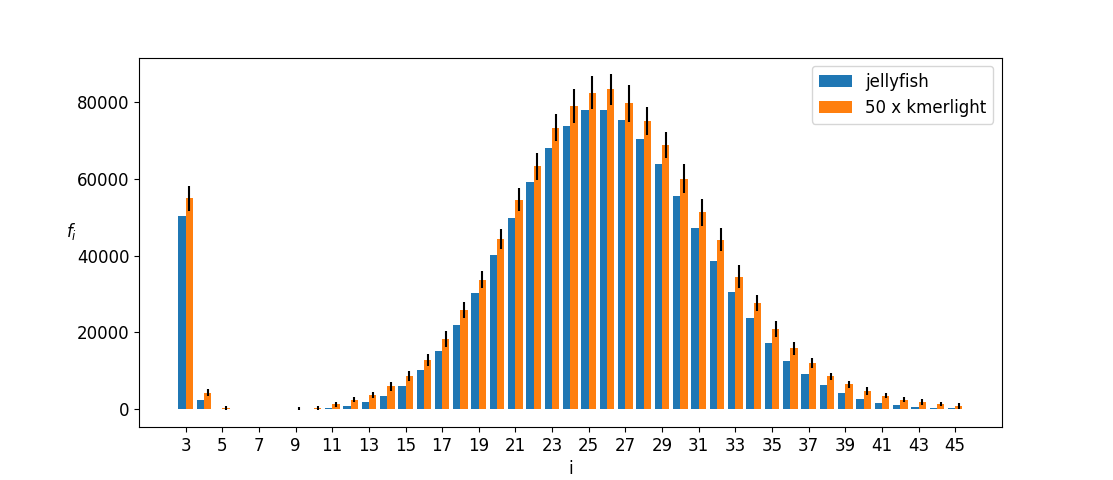
\includegraphics[width=1\textwidth, trim={1.5cm, 0cm, 2.5cm, 1.3cm}, clip]{{images/histogram_errors_L1000000_c50_e0.02_k21_normal}.png}}
\caption[Comparison of exact and approximated histograms]{Values of exact $f_i$ produced by
Jellyfish software (blue) and approximated values $\hat f_i$ produced by Kmerlight averaged
from 50 trials (orange). The errorbars express the standard deviation of each estimate. 
Note that columns for $i=1,2$ were trimmed, having values approximately $10^7, 10^6$ respectively.}
\label{img:exact-vs-approximated-histogram}
\end{figure}

\paragraph{Higher relative errors and higher relative variance with lower $f_i$}
Another characteristic of the errors is a trend of increasing relative variance and relative
error of the estimates for lower values $f_i$\footnote{Note that the absolute mean error
$(\hat f_i - f_i)$ and absolute variance decrease with decreasing $f_i$, as it can be
seen in Figure \ref{img:exact-vs-approximated-histogram}. However, if
the errors are considered proportionally to $f_i$, as $(\hat f_i - f_i)/f_i$, these relative
errors and their variances increase with decreasing $f_i$.}. In Figure \ref{img:relative-errors}
we visualize mean and standard deviation of relative errors $(\hat f_i - f_i) / f_i$ of $f_i$
estimates. Kmerlight guarantees bounded errors only for most frequent $k$-mers, those with
high $f_i/F_0$ ratio, but a theoretical quantitative analysis of the error distribution
was not presented in the previous work \cite{Sivadasan2016, Melsted2014}. 

We provide a quantitative estimate of the variance in section \ref{sec:estimation-variance} 
and then we use this knowledge to set Kmerlight's parameters to achieve
a desired error in \ref{sec:parameters-choice}.

\begin{figure}
\centerline{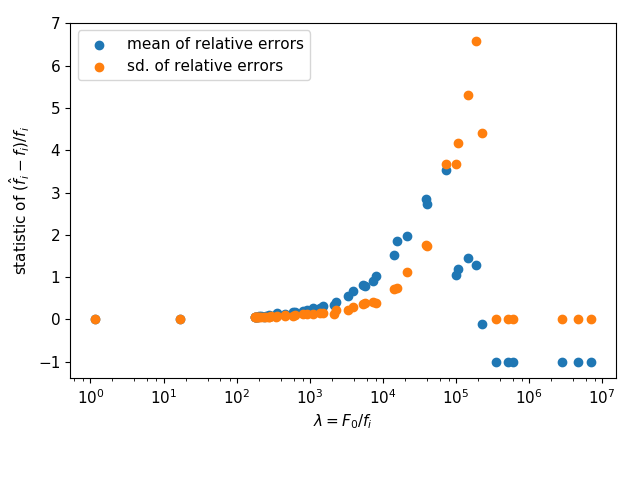
\includegraphics[width=0.8\textwidth, trim={0cm, 1.2cm, 0cm, 0cm}, clip]{{images/relative_errors_mean_std}.png}}
\caption[Relative approximation errors]{The mean and standard deviation of relative
errors $(\hat f_i - f_i) / f_i$ for columns sorted by decreasing $f_i$ (increasing $F_0/f_i$).
The drop in both statistics at values $\lambda = 10^5$ is caused by Kmerlight's 
insensitivity to infrequent $k$-mers.}
\label{img:relative-errors}
\end{figure}

\paragraph{Insensivity to Lowest $f_i$}
Since the hash tables of Kmerlight's sketch are smaller than the number of all $k$-mers,
many $k$-mers collide. When $f_i$, the number of distinct $k$-mers with abundance $i$, reaches
a specific boundary (in Figure \ref{img:exact-vs-approximated-histogram-log} it seems to be 
$5 \times 10^2$), the probability that at least one $k$-mer with abundance $i$ becomes stored
in a collision-free counter at any level approaches to zero.

As a result, the estimates $\hat f_i$ for the lowest $f_i$ may be based on none or
very few counters with value $i$. If no $k$-mer survives the collisions ($t_i = 0$)
then $\hat f_i = 0$. If very few $k$-mers survive the collisions, the estimator
multiplies the number collision-free counters by factor $2^{w^*}$ and the estimate may
overestimate $f_i$ drastically if a higher level $w^*$ was selected.

This effect is expected, but we point it out as it may limit the usage of the approximated
histogram to some applications.

\begin{figure}
\centerline{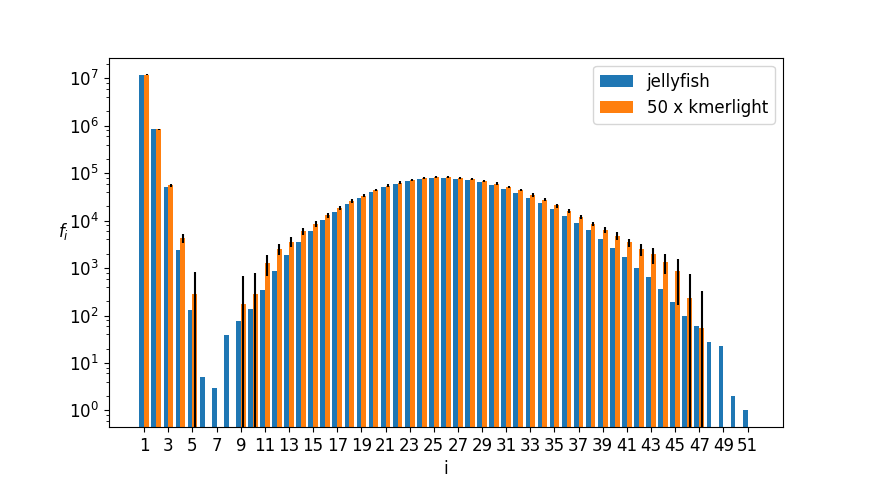
\includegraphics[width=1\textwidth, trim={1.5cm, 0cm, 2cm, 1.3cm}, clip]{{images/histogram_errors_L1000000_c50_e0.02_k21_normal_log}.png}}
\caption[Comparison of exact and approximated histograms in log scale]{Exact (blue) and
average approximated (orange) histograms, identical to those in figure 
\ref{img:exact-vs-approximated-histogram}, but displayed in a logarithmic scale with values 
$i=1, 2$ included. Note the lack of orange columns where blue columns reach lower 
values -- due to hashing collisions, Kmerlight cannot estimate $f_i$ lower than $5 \times 10^2$.}
\label{img:exact-vs-approximated-histogram-log}
\end{figure}

\subsection{Explanation of the Histogram Shape}
Kmerlight guarantees precise estimate of those $f_i$ that have with values close to $F_0$.
Unfortunately, in the sequencing data, sequencing errors often create many unique $k$-mers
and thus have $f_1$ close to $F_0$ and $f_i$ for $i > 1$ are much smaller than $F_0$. 

For example, with sequencing error rate of 2\%, 35\% occurences of $21$-mers are erroneous and thus
unique with high probability. As an effect 35\% of all input $k$-mers are concentrated in $f_1$ and
65\% of $k$-mers are distributed to other $f_i$. 

Furthermore, to increase $f_1$ by one, only one $k$-mer occurence is needed, but to increase
$f_{10}$ by one, ten error-free occurences of the same $k$-mer must be present in the input stream. 
As a result, less than 6.5\% of distinct $k$-mers have abundance greater than ten.

These effects explain, why the value of $f_1$ is approximately a hundred times larger than
the values of $f_i$ for $i>10$ in the presented experimental data in figures
\ref{img:exact-vs-approximated-histogram} and \ref{img:exact-vs-approximated-histogram-log}.
